\section{Software Realization}
\label{sec:software-realization}
To fully understand the ADRIAN protocol \cite{mann2023ADRIAN}, we have to implement a prototype of the protocol. This section describes the design and implementation of the ADRIAN protocol, as well as the experimental setup used to evaluate the protocol. The implementation is done in Java, and the source code can be found on GitHub\footnote{\url{https://github.com/jornverhoeven/thesis-project}}. 


\subsection{Overview}
\label{ssec:overview}
% \comment{Zoltan}{It would be a good to add an overview diagram that shows the structure of the while program on a higher level of abstraction than individual classes.}
To start things off we will give a brief overview of the components of the ADRIAN prototype. The component overview can be seen in Figure \ref{fig:adrian-component-overview}, and will be used as a reference throughout this section.

\begin{figure}[H]
    \centering
    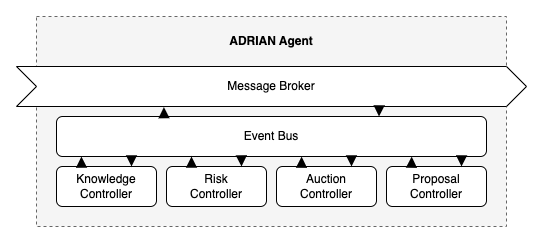
\includegraphics[width=0.8\textwidth]{_content/adrian-component-overview.png}
    \caption{Overview of the components of the ADRIAN protocol. The \code{MessageBroker} is responsible for interfacing with the external world, while the \code{EventBus} is used for internal communication. The \code{Controllers} are responsible for handling the different aspects of the agent, such as knowledge sharing and auctions. They are each responsible for a specific set of events and are connected to the event bus.}
    \label{fig:adrian-component-overview}
\end{figure}

For the architecture design of the prototype, we wanted to create something that is easy to understand, maintain, and instrument. To achieve this, we chose to implement an Event-Driven architecture. This architecture is based on the Observer pattern \cite{gamma1995design}, commonly used in software development. By sending messages through an event bus (See \code{EventBus} in figure \ref{fig:adrian-component-overview}), we can decouple the different components of the system. Next to being able to decouple the components, it also allows us to easily instrument the system. By listening to the events on the event bus during our experiments, we can count the number of events and the time between events. This allows us to easily collect metrics of the system. More on these metrics in Section \ref{ssec:metrics}.

Each controller in our design is responsible for a specific set of events and is connected to the event bus. This allows us to easily add new controllers, or replace existing ones during our experiments. The controllers are responsible for handling the different aspects of the agent. 

\begin{enumerate}
    \item The \code{KnowledgeController} is responsible for receiving and sharing knowledge. 
    \item The \code{RiskController} is responsible for detecting risks.
    \item The \code{AuctionController} is responsible for handling auctions. 
    \item The \code{ProposalController} is responsible for finding and applying proposals.
\end{enumerate}

We chose to detach the external communication from the internal communication. This allows us to easily replace the external communication with a different implementation. More on this in Section \ref{sssec:message-broker}.
The \code{MessageBroker} is the layer for interfacing with the external world. The \code{MessageBroker} is responsible for sending and receiving messages from other agents and dispatching them to the event bus.

\subsection{Class Diagrams}
\label{ssec:class-diagrams}
\addtocontents{toc}{\protect\setcounter{tocdepth}{2}}

In this section, we present an overview and analysis of a UML Class Diagram for our proposed implementation of the ADRIAN protocol \cite{mann2023ADRIAN} which can be seen in Figures \ref{fig:uml-agent} through \ref{fig:uml-services}. At a glance, the architecture features multiple controllers, connected through an internal event bus, and a message broker external communication. Additionally, some classes have been extended to support the experimental setup, which is further explained in Section \ref{sec:experiments}.

\begin{figure}[H]
    \centering
    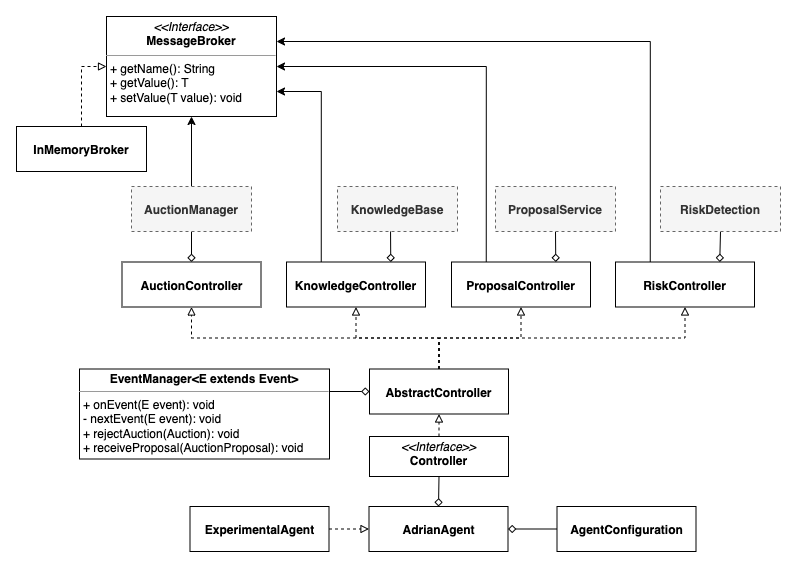
\includegraphics[width=0.8\textwidth]{_content/uml-agent}
    \caption{UML Diagram of the code structure of an Agent.}
    \label{fig:uml-agent}
\end{figure}

\subsubsection{Increased Cohesion and Reduced Coupling through Controller Interfaces}
\label{sssec:reduced-cohesion-coupling}
The systems architecture uses multiple controllers to handle various aspects of the agent, aiming to reduce both cohesion and coupling between components. Each controller is responsible for a specific set of tasks and the corresponding events, leading to a more modular and flexible design. This separation of functionality allows for easier maintenance, as well as the ability to replace controllers with new implementations, minimizing the impact on other parts of the system.

\subsubsection{Event Bus for internal communication}
\label{sssec:event-bus}
To enable communication between controllers, an internal event bus is created. The event bus is in essence nothing more than a Observer pattern (also known as \texttt{EventEmitter} or \texttt{Pup/Sub})\cite{gamma1995design}. This decouples the controllers from one another, as they are not directly aware of each other. Controllers can publish and subscribe to events on the event bus, and the event bus will then notify all subscribers when an event is published. 

\subsubsection{Controllers as an interfacing layer}
\label{sssec:controllers-interfacing-layer}
Controllers serve as an interfacing layer, between the event bus and the services responsible for the computations. This abstraction shields the services from the complexities of event handling, promoting modularity and reusability. It allows the services to be reused in other contexts and makes the code easier to test as it is not dependent on any external form of communication (which is handled by the controllers).

\subsubsection{Message Broker for external communication}
\label{sssec:message-broker}
The system uses a \code{MessageBroker} which facilitates communication between agents. It allows for both incoming and outgoing messages to be handled by the agent while abstracting away the underlying protocol. Incoming messages are processed and dispatched onto the internal event bus, triggering the relevant controllers to handle the message. On the other hand, outgoing messages are sent to the \code{MessageBroker}, which then sends the message to the appropriate agent.

\add{Rewrite the following paragraph to be easier to understand}
The \code{MessageBroker} as an interface can be concretized by different implementations, depending on hardware-/software-requirements. In the experimental setup, a single \code{MessageBroker} is used by all agents and works directly in memory. This avoids any additional network complexity and allows for easier simulation. In a real-world scenario, the \code{MessageBroker} would be a network service, which is used to send messages between agents over the network using HTTP requests or some other protocol such as MQTT. From the agent's perspective, the \code{MessageBroker} would be the same, regardless of the implementation, and thus reducing coupling between the agents and the underlying communication protocol.

\subsubsection{Similarities in graph data structures}
\label{sssec:graph-data-structures}
In the real world, the infrastructure is a graph structure, something that it \comment{Zoltan}{This could be interpreted in such a way that the speicific graph is hard-coded in the program. I think this is not what you want to say} captured in the code of the agent as well. The \code{Infrastructure}-graph consists of two types of nodes; \code{InfrastructureNode} and \code{SoftwareComponent}. These nodes can be mapped to actual hardware (e.g. Servers and IoT devices) and software (e.g. Databases and Services) in real-world applications, their concrete implementation is intentionally left away to reduce overhead and complexity.

\begin{figure}[H]
    \centering
    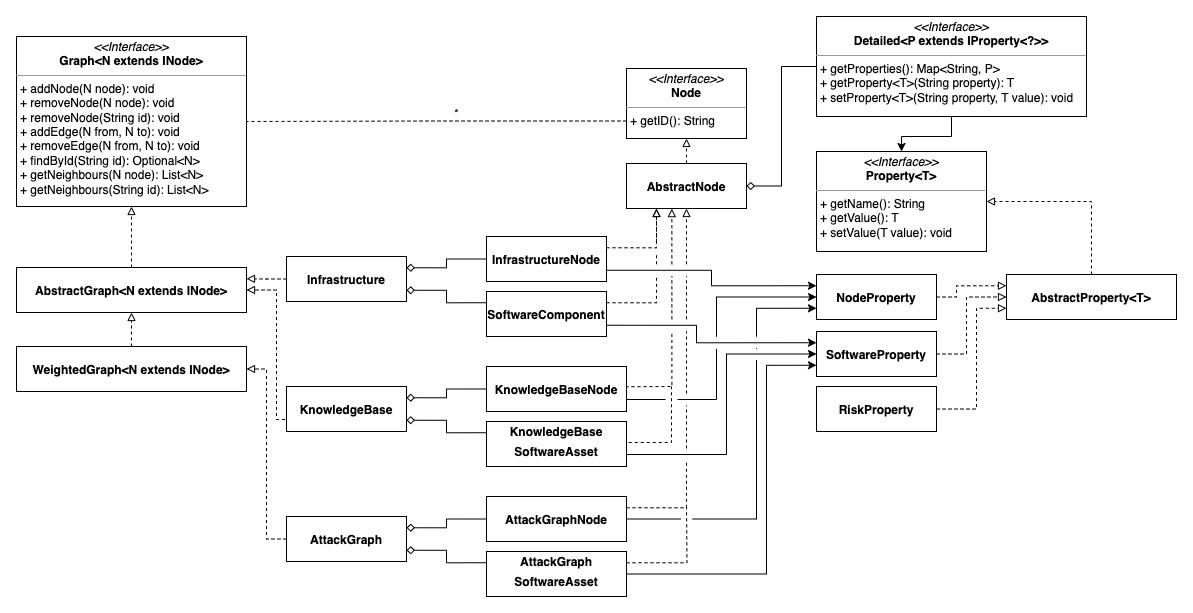
\includegraphics[width=1.2\textwidth]{_content/uml-graphs}
    \caption{UML Diagram explaining the structure of the Graphs, in a way that the separate classes are similar to their counterparts.}
    \label{fig:uml-graphs}
\end{figure}

\subsubsection{Services}
\label{sssec:services}
Each controller is only responsible for converting events into service calls. But to implement the actual logic, the controllers use services. These services are responsible for the actual computations, such as calculating the \code{AttackGraphs} or finding \code{Proposal}s. Figure \ref{fig:uml-services} shows how the services are tied together.

\begin{figure}[H]
    \centering
    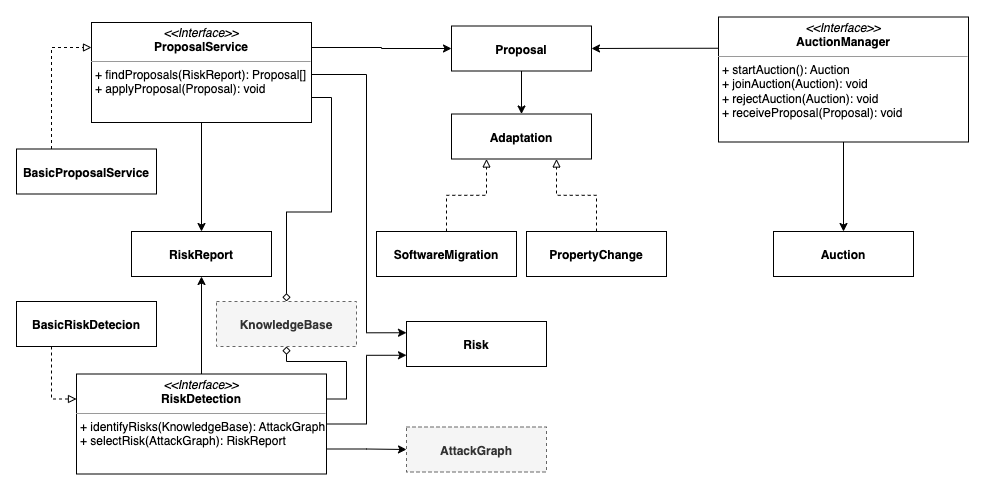
\includegraphics[width=1.0\textwidth]{_content/uml-services}
    \caption{UML Diagram depicting how the Agent's services are tied together.}
    \label{fig:uml-services}
\end{figure}

\begin{description}
    \item[RiskDetection] This service is responsible for detecting risks in the infrastructure. It does this by calculating the attack graph for each node in the infrastructure. With the attack graph, it can then identify \textit{Critical Paths} by finding paths from nodes to a \textit{critical software component}. These \textit{Critical Paths} are then used to calculate the risk damage value. We calculate the risk damage by taking the potential damage value of a software component and multiplying it by the probability of the path. The probability is calculated over all edges between nodes, that are in the same direction of the critical path. 
    \begin{figure}[H]
        \centering
        \begin{subfigure}[b]{0.4\textwidth}
            \centering
            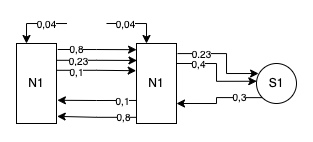
\includegraphics[width=\textwidth]{_content/attack-graph.png}
            \caption{Attack graph between nodes and software components}
            \label{fig:attack-graph}
        \end{subfigure}
        \hspace{0.5cm}
        \centering
        \begin{subfigure}[b]{0.4\textwidth}
            \centering
            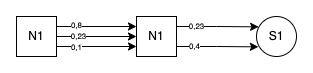
\includegraphics[width=\textwidth]{_content/riskreport-future-research-a.png}
            \caption{Risk report for a critical path}
            \label{fig:risk-report}
        \end{subfigure}
        \caption{On the left is the graph representation of an attack graph, where each edge is a risk that holds a probability of an attacker exploiting it. The graph is directional and can hold edges in multiple directions. On the right is the graph representation of a risk report. The risk report is also directional but only contains the edges that are in the same \textit{direction} as the critical path. Both graphs can have incoming edges to indicate that a node could be the starting point of an attack.}
    \end{figure}

    \item[ProposalService] This service is responsible for calculating proposals that the node is willing to apply. It does this by taking the risk report from an auction and applying different adaptations to it. For example, an adaptation could be to update the properties of a node or software or migrate a software component to another node. The service then calculates the risk damage value for each adaptation and returns the adaptation with the lowest risk damage value. This adaptation is then used as a bid in the auction, for the auctioneer to consider. 
    
    \item[AuctionManager] This service is responsible for starting and managing the state of an auction. When it starts a new auction, it will send invitations to other agents and wait for their replies (accept or reject). It will also keep track of the current state of the auction and wait for proposals to be submitted. When a proposal is submitted, it will check if all participating nodes replied. If this is the case, it will calculate the risk damage value for each proposal, and select the proposal with the lowest risk damage value. This proposal is then broadcast to all participating nodes, and the auction is finished. The manager will then wait for the next auction to start. There might also be cases where participating nodes fail to send proposals. For these cases, the \code{AuctionManager} has a timeout that starts when an auction starts. If the timeout is reached, the manager will finish the auction at that point, and select the proposal with the lowest risk damage value. If no applicable proposals are received, the auction is canceled and nothing is done.
\end{description}

% \subsection{Sequence Diagrams}
% \label{ssec:sequence-diagrams}
% \add{Update text or remove section}
% \begin{figure}[H]
%     \centering
%     \includegraphics[width=0.8\textwidth]{_content/knowledge-sharing}
%     \caption{Knowledge Exchange Sequence Diagram}
%     \label{fig:knowledge-sharing}
% \end{figure}

% \begin{figure}[H]
%     \centering
%     \includegraphics[width=0.8\textwidth]{_content/auction}
%     \caption{Auction Sequence Diagram}
%     \label{fig:auction}
% \end{figure}

% \addtocontents{toc}{\protect\setcounter{tocdepth}{3}}
